\documentclass[12pt]{article}
\usepackage[margin=.8in]{geometry}
\usepackage{float}
\usepackage{multicol}
\usepackage{lmodern}
\usepackage{amssymb,amsmath}
\usepackage{ifxetex,ifluatex}
\usepackage{fixltx2e} % provides \textsubscript
\ifnum 0\ifxetex 1\fi\ifluatex 1\fi=0 % if pdftex
  \usepackage[T1]{fontenc}
  \usepackage[utf8]{inputenc}
\else % if luatex or xelatex
  \ifxetex
    \usepackage{mathspec}
    \usepackage{xltxtra,xunicode}
  \else
    \usepackage{fontspec}
  \fi
  \defaultfontfeatures{Mapping=tex-text,Scale=MatchLowercase}
  \newcommand{\euro}{€}
\fi
% use upquote if available, for straight quotes in verbatim environments
\IfFileExists{upquote.sty}{\usepackage{upquote}}{}
% use microtype if available
\IfFileExists{microtype.sty}{%
\usepackage{microtype}
\UseMicrotypeSet[protrusion]{basicmath} % disable protrusion for tt fonts
}{}
\usepackage{longtable,booktabs}
\usepackage{graphicx}
\makeatletter
\def\maxwidth{\ifdim\Gin@nat@width>\linewidth\linewidth\else\Gin@nat@width\fi}
\def\maxheight{\ifdim\Gin@nat@height>\textheight\textheight\else\Gin@nat@height\fi}
\makeatother
% Scale images if necessary, so that they will not overflow the page
% margins by default, and it is still possible to overwrite the defaults
% using explicit options in \includegraphics[width=4in][width, height, ...]{}
\setkeys{Gin}{width=\maxwidth,height=\maxheight,keepaspectratio}
\ifxetex
  \usepackage[setpagesize=false, % page size defined by xetex
              unicode=false, % unicode breaks when used with xetex
              xetex]{hyperref}
\else
  \usepackage[unicode=true]{hyperref}
\fi
\hypersetup{breaklinks=true,
            bookmarks=true,
            pdfauthor={Brandon LeBeau},
            pdftitle={PSQF 4143: Section 3},
            colorlinks=true,
            citecolor=blue,
            urlcolor=blue,
            linkcolor=magenta,
            pdfborder={0 0 0}}
\urlstyle{same}  % don't use monospace font for urls
\setlength{\parindent}{0pt}
\setlength{\parskip}{6pt plus 2pt minus 1pt}
\setlength{\emergencystretch}{3em}  % prevent overfull lines
\setcounter{secnumdepth}{0}

\title{PSQF 4143: Section 3}
\author{Brandon LeBeau}
\date{}

\begin{document}
\maketitle

\section{Statistics vs Parameters}\label{statistics-vs-parameters}

\begin{itemize}
\itemsep1pt\parskip0pt\parsep0pt
\item
  \emph{Statistics} - A number that describes the sample; hopefully a
  representative number for the population

  \begin{itemize}
  \itemsep1pt\parskip0pt\parsep0pt
  \item
    Notation: An English letter (i.e. \(X\), \(\bar{X}\))
  \end{itemize}
\item
  \emph{Parameter} - A number to describe the population (i.e.~the true
  value)

  \begin{itemize}
  \itemsep1pt\parskip0pt\parsep0pt
  \item
    Notation: A Greek letter (i.e. \(\mu\), \(\sigma\))
  \end{itemize}
\end{itemize}

\section{Notation}\label{notation}

\begin{itemize}
\itemsep1pt\parskip0pt\parsep0pt
\item
  An observed data point is represented with a capital letter, commonly
  \(X\). This would represent the value for a single individual.

  \begin{itemize}
  \itemsep1pt\parskip0pt\parsep0pt
  \item
    Example: X = 25
  \end{itemize}
\item
  Little \(x\) is used for a deviation score.
\item
  The number of subjects in the population is denoted with a capital
  \(N\). The number in the sample is denoted with a small \(n\).
\item
  If there are multiple observations or groups a subcript is used.

  \begin{itemize}
  \itemsep1pt\parskip0pt\parsep0pt
  \item
    Example: A sample of 3 observations (n = 3): \(X_{1} = 12\),
    \(X_{2} = 23\), \(X_{3} = 8\).
  \end{itemize}
\end{itemize}

\section{Notation 2}\label{notation-2}

\begin{itemize}
\itemsep1pt\parskip0pt\parsep0pt
\item
  The greek captial letter, \(\Sigma\), is used to indicate summation.

  \begin{itemize}
  \itemsep1pt\parskip0pt\parsep0pt
  \item
    More formally:
    \(\displaystyle \sum^{n}_{i=1} X_{i} = X_{1} + X_{2} + ... + X_{n}\)
  \item
    This means sum the value of \(X\) from 1 to \(n\).
  \end{itemize}
\item
  Example: \(X_{1} = 12\), \(X_{2} = 23\), \(X_{3} = 8\).
  \[ \displaystyle \sum_{i=1}^{n} X_{i} = 12 + 23 + 8 = 43  \]
\end{itemize}

\section{Single number Descriptive
Statistics}\label{single-number-descriptive-statistics}

\begin{itemize}
\itemsep1pt\parskip0pt\parsep0pt
\item
  \emph{Central Tendency} - a set of descriptive statistics that
  describes a data set in a single number; also known as measures of
  central tendency as they describe where the center of the distribution
  lies

  \begin{itemize}
  \itemsep1pt\parskip0pt\parsep0pt
  \item
    Mode
  \item
    Median
  \item
    Mean (Average)
  \end{itemize}
\end{itemize}

\section{Measure of Central Tendency}\label{measure-of-central-tendency}

\begin{itemize}
\itemsep1pt\parskip0pt\parsep0pt
\item
  Mode:

  \begin{itemize}
  \itemsep1pt\parskip0pt\parsep0pt
  \item
    Indicates the most frequent value/category in the distribution.
  \end{itemize}
\item
  Calculating the mode:

  \begin{itemize}
  \itemsep1pt\parskip0pt\parsep0pt
  \item
    Discrete Data: Value with the greatest frequency.
  \item
    Categorized Continuous Data (i.e.~Frequency Table): Midpoint of the
    interval with the greatest frequency.
  \item
    Continuous Data: The highest point of the frequency distribution.
  \end{itemize}
\end{itemize}

\section{Mode Calculations}\label{mode-calculations}

\begin{figure}[H]
\centering
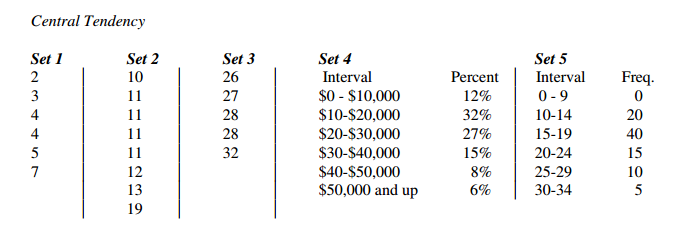
\includegraphics[width=4in]{PracticeCentralTend.png}
\caption{Practice Central Tendency}
\end{figure}

\section{Measure of Central Tendency
2}\label{measure-of-central-tendency-2}

\begin{itemize}
\itemsep1pt\parskip0pt\parsep0pt
\item
  Median:

  \begin{itemize}
  \itemsep1pt\parskip0pt\parsep0pt
  \item
    Is the value where half of the data fall above and half fall below.
  \end{itemize}
\item
  Calculating the median:

  \begin{itemize}
  \itemsep1pt\parskip0pt\parsep0pt
  \item
    Nominal Data: Cannot be done meaningfully
  \item
    Discrete Data:

    \begin{enumerate}
    \def\labelenumi{\arabic{enumi}.}
    \itemsep1pt\parskip0pt\parsep0pt
    \item
      Order values from highest to lowest, find the middle value.
    \item
      Alternatively: find the value: \[ L = \frac{n+1}{2} \]

      \begin{itemize}
      \itemsep1pt\parskip0pt\parsep0pt
      \item
        If L is a whole number, the median is the Lth value
      \item
        If L is a decimal, the median is the average between the two
        values around L (i.e.~the value rounded up and down from L)
      \end{itemize}
    \end{enumerate}
  \end{itemize}
\end{itemize}

\section{Measure of Central Tendency
2}\label{measure-of-central-tendency-2-1}

\begin{itemize}
\itemsep1pt\parskip0pt\parsep0pt
\item
  Calculating the median:

  \begin{itemize}
  \itemsep1pt\parskip0pt\parsep0pt
  \item
    Continuous Data:

    \begin{itemize}
    \itemsep1pt\parskip0pt\parsep0pt
    \item
      determine where in the interval the median falls as a fraction,
      then go that fraction from the interval's lower limit to its upper
      limit
    \item
      \[ Median = L + \frac{ \frac{n}{2} - f_{below}}{f_{at}} * w \]
      Where \(L\) is the lower limit of the of the interval containing
      the median \(n\) is total frequency \(f_{below}\) is the frequency
      below the interval \(f_{at}\) is the frequency at the interval
      \(w\) is the bin width
    \end{itemize}
  \end{itemize}
\end{itemize}

\section{Median Calculations}\label{median-calculations}
\begin{multicols}{3}
2\\3\\4\\4\\5\\7

\columnbreak
10\\11\\11\\11\\11\\12\\13\\19

\columnbreak
26\\27\\28\\28\\32

\end{multicols}

\begin{multicols}{2}
\begin{longtable}[c]{@{}ll@{}}
\toprule
Interval & Percent\tabularnewline
\midrule
\endhead
\$0-\$10000 & 12\%\tabularnewline
\$10000-\$20000 & 32\%\tabularnewline
\$20000-\$30000 & 27\%\tabularnewline
\$30000-\$40000 & 15\%\tabularnewline
\$40000-\$50000 & 8\%\tabularnewline
\$50000 and up & 6\%\tabularnewline
\bottomrule
\end{longtable}

\columnbreak
\begin{longtable}[c]{@{}ll@{}}
\toprule
Interval & Percent\tabularnewline
\midrule
\endhead
0 - 9 & 0\tabularnewline
10 - 14 & 20\tabularnewline
15 - 19 & 40\tabularnewline
20 - 24 & 15\tabularnewline
25 - 29 & 10\tabularnewline
30 - 34 & 5\tabularnewline
\bottomrule
\end{longtable}
\end{multicols}

\newpage
\section{Measures of Central Tendency
3}\label{measures-of-central-tendency-3}

\begin{itemize}
\itemsep1pt\parskip0pt\parsep0pt
\item
  Mean:

  \begin{itemize}
  \itemsep1pt\parskip0pt\parsep0pt
  \item
    Is the average of the data, also known as the ``balance point'' or
    the place where the distribution would balance on a fulcrum.
  \item
    The mean is used for interval or ratio data and the value is
    interpretted in the same metric as the raw data.
  \end{itemize}
\item
  Notation:

  \begin{itemize}
  \itemsep1pt\parskip0pt\parsep0pt
  \item
    Sample: \(\bar{X}\) - called ``X-bar''
  \item
    Population: \(\mu\) - Greek letter ``mu''
  \end{itemize}
\end{itemize}

\section{Measures of Central Tendency
3}\label{measures-of-central-tendency-3-1}

\begin{itemize}
\itemsep1pt\parskip0pt\parsep0pt
\item
  Calculating the Mean

  \begin{itemize}
  \itemsep1pt\parskip0pt\parsep0pt
  \item
    Sample:
    \[\bar{X} = \frac{\sum X}{n} = \frac{X_{1} + X_{2} + ...}{n} \]
  \item
    Population:
    \[\mu = \frac{\sum X}{N} = \frac{X_{1} + X_{2} + ...}{N} \]
  \end{itemize}
\end{itemize}

\section{Mean Calculations 1}\label{mean-calculations-1}

2\\3\\4\\4\\5\\7

\section{Mean Comic}\label{mean-comic}

\begin{figure}[H]
\centering
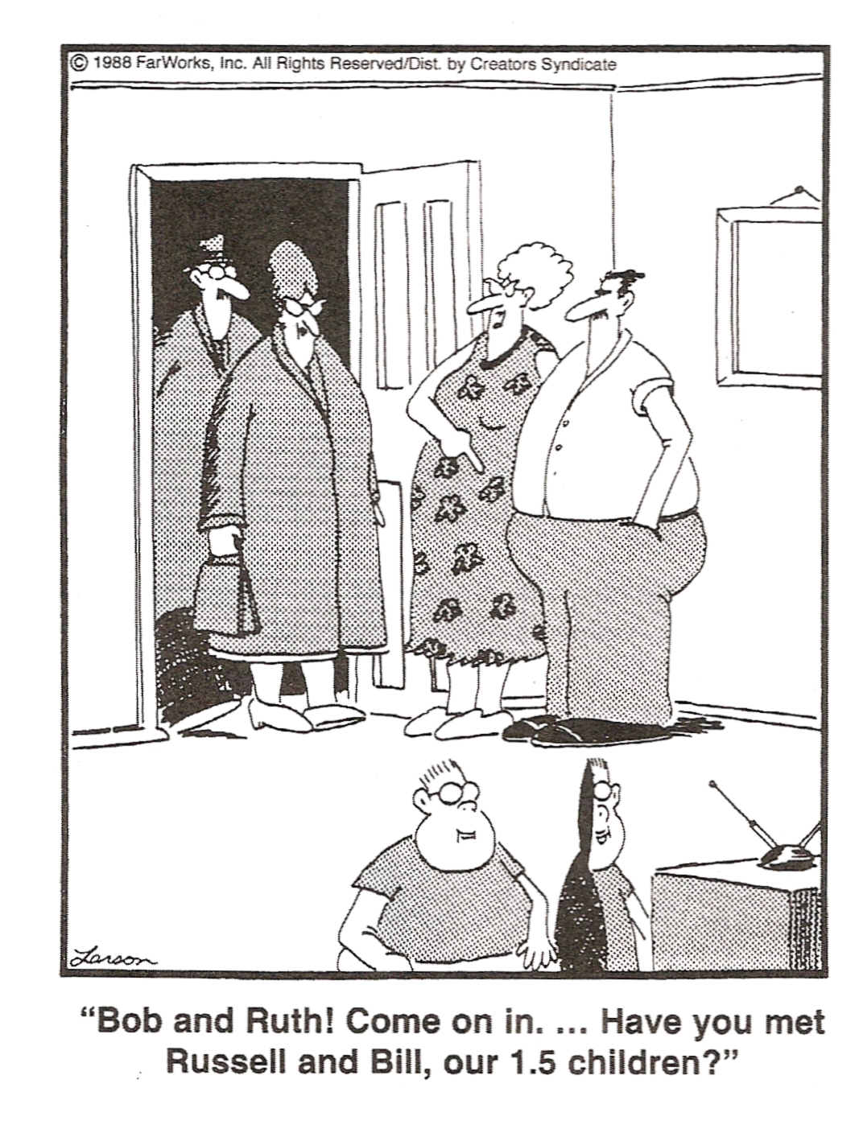
\includegraphics[width=3in]{farside.png}
\caption{Comic}
\end{figure}

\section{Measures of Central Tendency
3}\label{measures-of-central-tendency-3-2}

\begin{itemize}
\itemsep1pt\parskip0pt\parsep0pt
\item
  Calculating the Mean

  \begin{itemize}
  \itemsep1pt\parskip0pt\parsep0pt
  \item
    Categorized Data (Frequency Table):
    \[ \bar{X} = \frac{\sum f * X_{midpoint}}{\sum f} \] where \(f\) and
    \(X_{midpoint}\) are the frequency and midpoint of each bin/class.
  \end{itemize}
\end{itemize}

\section{Mean Calculations 2}\label{mean-calculations-2}
\begin{multicols}{2}
\begin{longtable}[c]{@{}ll@{}}
\toprule
Interval & Percent\tabularnewline
\midrule
\endhead
0 - 9 & 0\tabularnewline
10 - 14 & 20\tabularnewline
15 - 19 & 40\tabularnewline
20 - 24 & 15\tabularnewline
25 - 29 & 10\tabularnewline
30 - 34 & 5\tabularnewline
\bottomrule
\end{longtable}

\columnbreak
\begin{longtable}[c]{@{}ll@{}}
\toprule
Interval & Percent\tabularnewline
\midrule
\endhead
\$0-\$10000 & 12\%\tabularnewline
\$10000-\$20000 & 32\%\tabularnewline
\$20000-\$30000 & 27\%\tabularnewline
\$30000-\$40000 & 15\%\tabularnewline
\$40000-\$50000 & 8\%\tabularnewline
\$50000 and up & 6\%\tabularnewline
\bottomrule
\end{longtable}
\end{multicols}

\newpage
\section{Mean is Mathematically
Tractable}\label{mean-is-mathematically-tractable}

\begin{itemize}
\itemsep1pt\parskip0pt\parsep0pt
\item
  This is fancy math lingo meaning that the mean is able to be
  manipulated algebraicly.
\item
  Proof:
\end{itemize}

\[\frac{\sum X}{n} = \bar{X}\] \[n \frac{\sum X}{n} = n \bar{X}\]
\[\sum X = n \bar{X}\]

\section{Weighted Mean}\label{weighted-mean}

\begin{itemize}
\itemsep1pt\parskip0pt\parsep0pt
\item
  Used when groups are different sizes.
\end{itemize}

\[ \bar{X} = \frac{n_{a}\bar{X}_{a} + n_{b}\bar{X}_{b} + n_{c}\bar{X}_{c}}{n_{a} + n_{b} + n_{c}} \]

\begin{itemize}
\itemsep1pt\parskip0pt\parsep0pt
\item
  More generally:
\end{itemize}

\[ \bar{X} = \frac{\sum n_{j} \bar{X}_{j}}{\sum n_{j}} \]

\section{Weighted Mean Example}\label{weighted-mean-example}

Boys: 5, 8, 3, 7, 7 \\ Girls: 10, 12, 16, 8, 4, 8

\section{Weighted Mean Example 2}\label{weighted-mean-example-2}

District 1: n = 3347; Mean = 78.4\\District 2: n = 200; Mean =
52.8\\District 3: n = 334; Mean = 55.2

\section{Puzzler - Simpson's Paradox}\label{puzzler---simpsons-paradox}

\begin{itemize}
\itemsep1pt\parskip0pt\parsep0pt
\item
  The boys at Elm have a higher mean than the boys at Oak.
\item
  The girls at Elm have a higher mean than the girls at Oak.
\item
  The combined mean at Elm is lower than the combined mean at Oak.
\end{itemize}

\section{Choosing a Statistic}\label{choosing-a-statistic}

\begin{itemize}
\itemsep1pt\parskip0pt\parsep0pt
\item
  What statistic would you choose if the distribution was normally
  distributed? Why?
\item
  What if the distribution was skewed?
\end{itemize}

\section{What to use for skewed
distributions?}\label{what-to-use-for-skewed-distributions}

Suppose we have the following distribution:


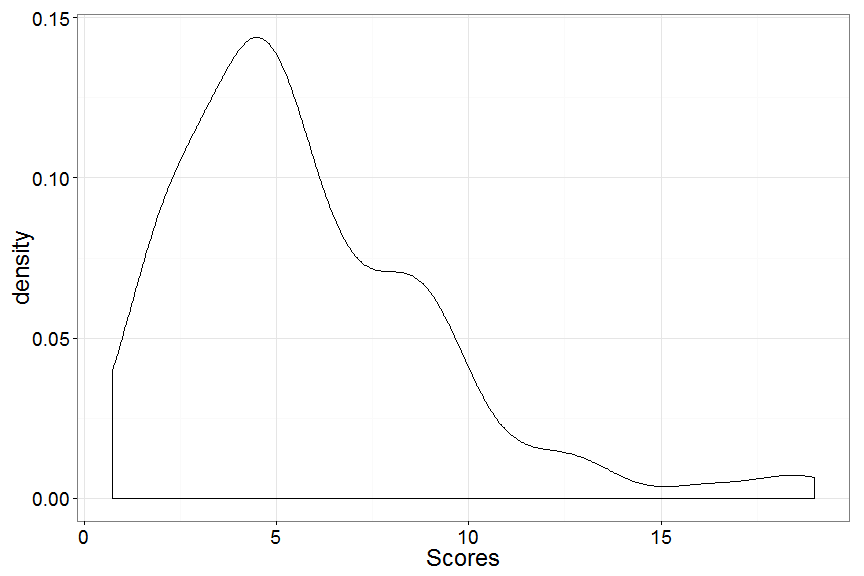
\includegraphics[width=3.5in]{figure/chisq-1.png}
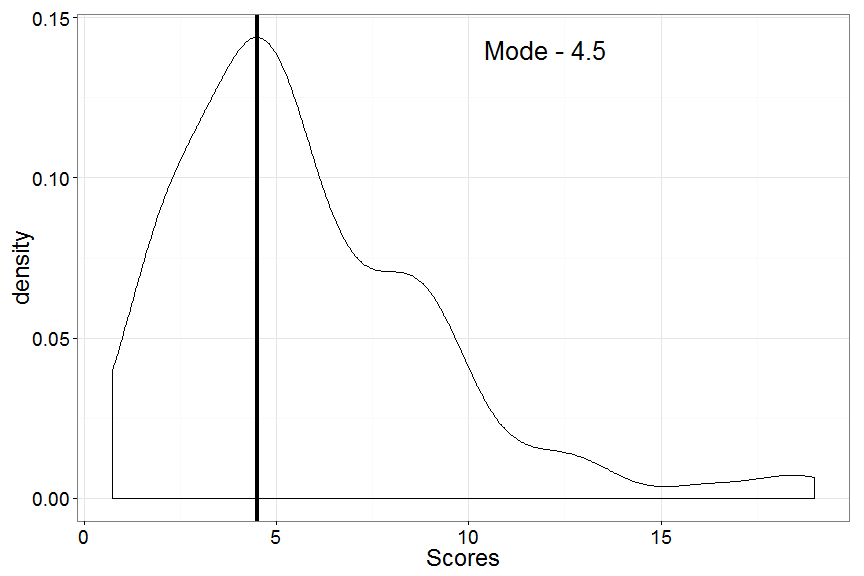
\includegraphics[width=3.5in]{figure/chisqmode-1.png} \\
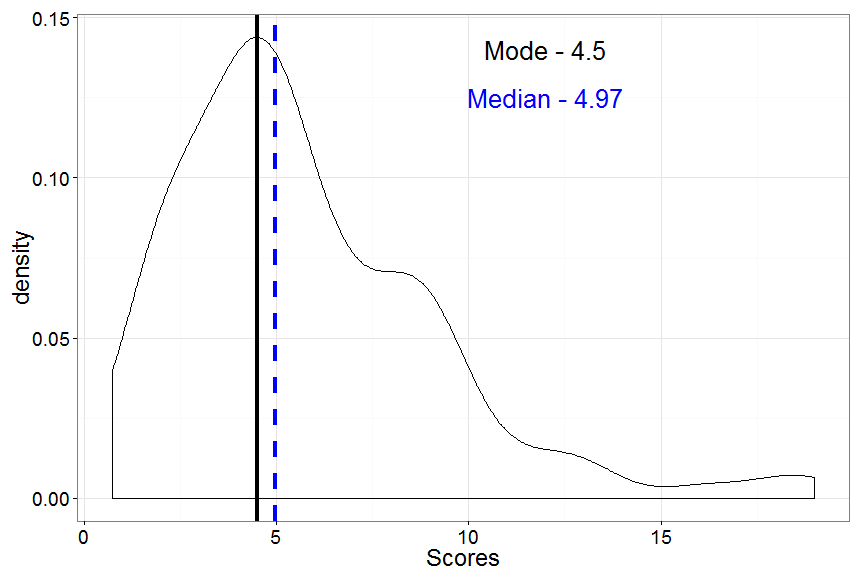
\includegraphics[width=3.5in]{figure/chisqmed-1.png}
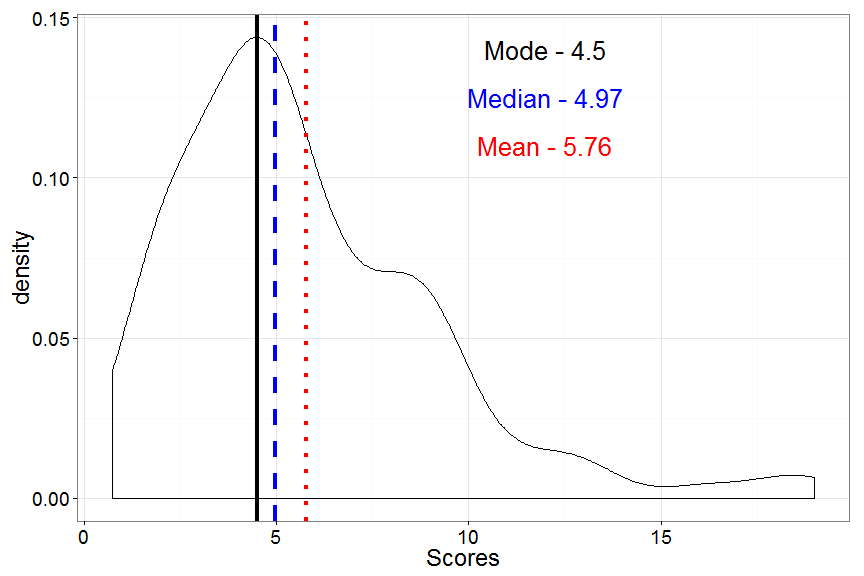
\includegraphics[width=3.5in]{figure/chisqmean-1.png}


\section{Strengths/Weaknesses of the
Mode}\label{strengthsweaknesses-of-the-mode}

\begin{itemize}
\itemsep1pt\parskip0pt\parsep0pt
\item
  Strengths:

  \begin{itemize}
  \itemsep1pt\parskip0pt\parsep0pt
  \item
    The mode is simple, easy to compute, and can be used with
    qualitative variables.
  \end{itemize}
\item
  Weaknesses:

  \begin{itemize}
  \itemsep1pt\parskip0pt\parsep0pt
  \item
    However, it can change easily or be undefined for multimodal data.

    \begin{itemize}
    \itemsep1pt\parskip0pt\parsep0pt
    \item
      This is often called sampling stability.
    \end{itemize}
  \item
    Not mathematically tractable.
  \end{itemize}
\end{itemize}

\section{Strengths/Weaknesses of the
Median}\label{strengthsweaknesses-of-the-median}

\begin{itemize}
\itemsep1pt\parskip0pt\parsep0pt
\item
  Strengths:

  \begin{itemize}
  \itemsep1pt\parskip0pt\parsep0pt
  \item
    The median is the most typical number in the distribution.

    \begin{itemize}
    \itemsep1pt\parskip0pt\parsep0pt
    \item
      The median minimizes \(\sum |X - Mdn| \leq \sum |X - c|\) where c
      is any other value.
    \item
      As such, the median is commonly used with income or prices.
    \end{itemize}
  \item
    The median is not affected by outliers

    \begin{itemize}
    \itemsep1pt\parskip0pt\parsep0pt
    \item
      This is due to the median is not based on the value of the scores,
      but rather the ranking of scores.
    \item
      The median would only be affected if the ranking of scores would
      change.
    \end{itemize}
  \item
    Easy to compute and computed for open-ended groups.
  \item
    Is the 50th percentile
  \end{itemize}
\item
  Weaknesses:

  \begin{itemize}
  \itemsep1pt\parskip0pt\parsep0pt
  \item
    Poor sampling stability compared to the mean (better than the mode).
  \item
    Not as mathematically tractable compared to the mean.
  \item
    Does not use all data in the calculation.
  \item
    Can not be calculated for qualitative data
  \end{itemize}
\end{itemize}

\section{Strengths/Weaknesses of the
Mean}\label{strengthsweaknesses-of-the-mean}

\begin{itemize}
\itemsep1pt\parskip0pt\parsep0pt
\item
  Strengths:

  \begin{itemize}
  \itemsep1pt\parskip0pt\parsep0pt
  \item
    Mathematically tractable

    \begin{itemize}
    \itemsep1pt\parskip0pt\parsep0pt
    \item
      Sum of deviation scores equals 0 (\(\sum(X - \bar{X}) = 0\))
    \item
      Minimizes the sum of squared deviations scores
      (\(\sum(X - \bar{X})^2\))
    \end{itemize}
  \item
    The mathematic properties make the mean the balance point of the
    distribution.
  \item
    Takes into account value of all numbers in the distribution.
  \item
    Used in many advanced statistical techniques.
  \end{itemize}
\item
  Weaknesses:

  \begin{itemize}
  \itemsep1pt\parskip0pt\parsep0pt
  \item
    Sensitive to outliers
  \item
    Unable to calculate for open-ended groups.
  \item
    Can not be calculated for qualitative data
  \end{itemize}
\end{itemize}

\end{document}
